%%%%%%%%%%%%
%file with comparative plots for SNe 
%%%%%%%%%%%%

\documentclass{article}
\usepackage{graphicx}

\begin{document}
\title{$i$-band second maximum: CSP Spectra}
\maketitle
This document contains optical spectra before and during the second maximum for three SNe: 2005am, 2007on, 2007al. The first SN is a normal Ia, whereas 2007on has a $\Delta m_{15}$ of 1.65 mag. 2007al is classified as a 91bg-like SN.
SN2005am has a second peak at $\sim$ 21$\,$d, 2007on at $\sim$ +15$\,$d whereas 2007al doesnt show a second peak.
\begin{figure}
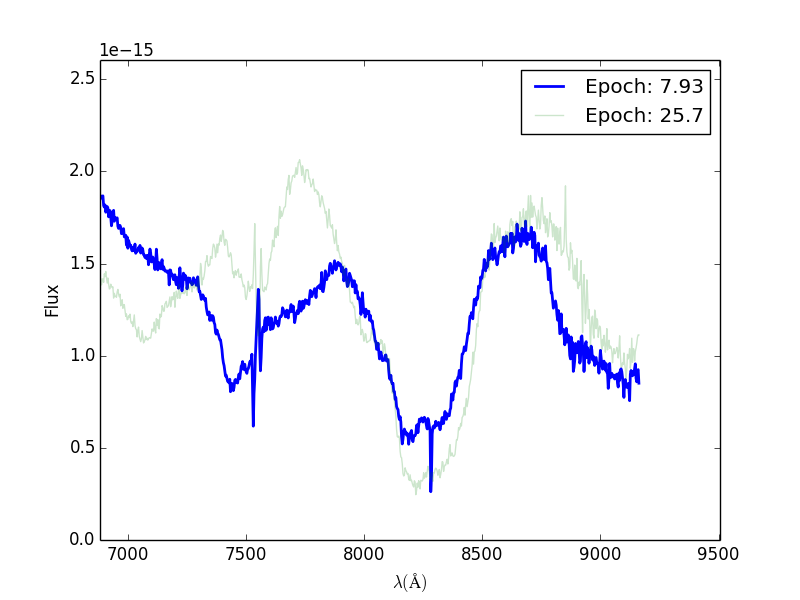
\includegraphics[width=.7\textwidth]{../img/05am_cspspec.png}
\caption{Two spectra for SN2005am from the CSP are plotted. \emph{Blue} Spectrum before the second maximum \emph{Green} Spectrum during. The Fe [II] feature appears to be clearly visible}
\end{figure}

\begin{figure}
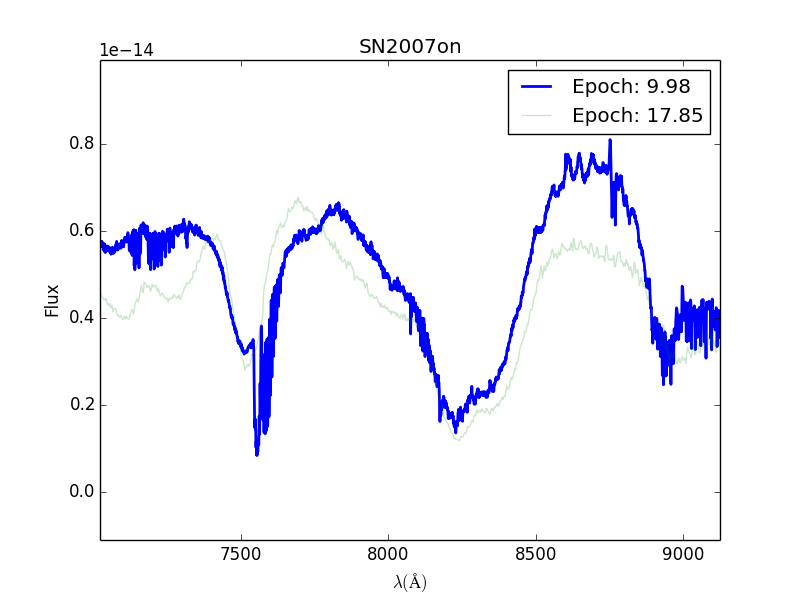
\includegraphics[width=.7\textwidth]{../img/07on_cspspec.png}
\caption{\emph{Blue}: Spectrum before the second maximum. \emph{Green}: spectrum during. The Fe [II] feature appears to be less prominent}
\end{figure}


\begin{figure}
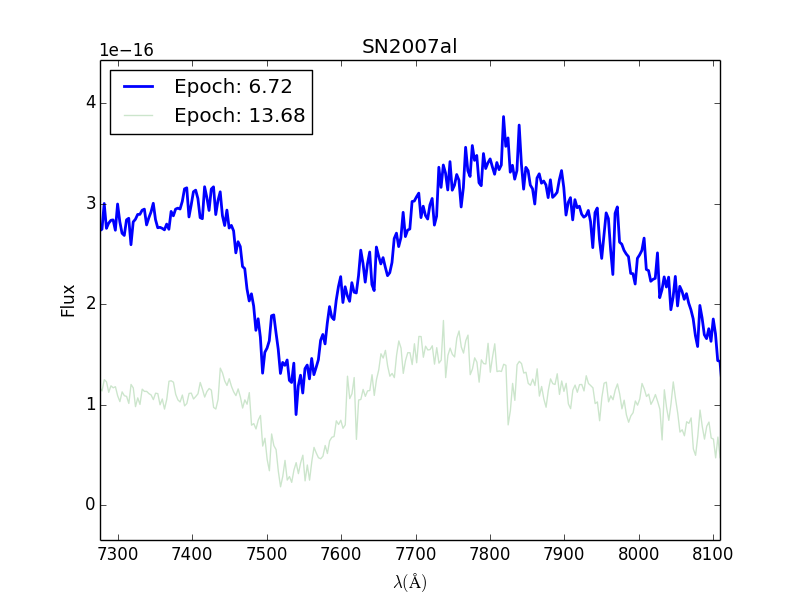
\includegraphics[width=.7\textwidth]{../img/07al_cspspec.png}
\caption{\emph{Blue}: Spectrum before the second maximum. \emph{Green}: spectrum during.}
\end{figure}

\end{document}
